\documentclass[dvipdfmx]{beamer}
\usepackage{bxdpx-beamer}% dvipdfmxなので必要
\usepackage{pxjahyper}% 日本語で'しおり'したい
%\documentclass[ckj]{beamer}
%\usepackage{etex}
%\usetheme{Warsaw}
\usetheme{Malmoe}
%\usetheme{AnnArbor}
%\usetheme{Hannover}
%\usetheme{Bergen}
%\usetheme{Berlin}
%\usetheme{Singapore}
%\usetheme{Montpellier}
%\usetheme{Pittsburgh}
\usepackage{tikz}
\usetikzlibrary{calc}
\usepackage{graphicx}
\usepackage{latexsym,amssymb}
%\usepackage{epsbox}
%\usepackage{multirow}
\usepackage{fancybox}
\usepackage{fancyvrb}
%\usepackage{listings}
\usepackage{tabularx} %\usepackage{pstricks,pst-node,pst-tree}
%\usepackage{multimedia}
%\usepackage{pstricks,pst-node,pst-tree}
%\usepackage{pst-all}
%\include{prooftree}
%\lstloadlanguages{pascal}
\renewcommand{\kanjifamilydefault}{\gtdefault}
\renewcommand{\familydefault}{\sfdefault}

\newcommand{\greentext}[1]{{\color[rgb]{0,0.5,0}{#1}}}
\newcommand{\redtext}[1]{{\color[rgb]{0.8,0,0}{#1}}}
\newcommand{\bluetext}[1]{{\color[rgb]{0,0,0.8}{#1}}}

\newcommand{\tuple}[1]{\langle{#1}\rangle}

\newcommand{\First}{\mathsf{First}_1}
\newcommand{\Follow}{\mathsf{Follow}_1}

%%pdt simulation

\newcommand{\pdtline}[6]{%
    \uncover<#6->{
    \node at (${#5}*(0,-.3)+(0,.3)$) {$\vdash$};%
    \node at (${#5}*(0,-.3)+(1.5,.3)$) {\parbox{12em}{(#1,}};%
    \node at (${#5}*(0,-.3)+(4.5,.3)$) {\parbox{10em}{#2,}};%
    \node at (${#5}*(0,-.3)+(5.7,.3)$) {\parbox{10em}{#3)}};%
    \node at (${#5}*(0,-.3)+(8,.3)$) {\parbox{20em}{#4}};%
    }
}

\newcommand{\initpdtline}[6]{%
    \uncover<#6->{
    \node at (${#5}*(0,-.3)+(1.5,.3)$) {\parbox{12em}{(#1,}};%
    \node at (${#5}*(0,-.3)+(4.5,.3)$) {\parbox{10em}{#2,}};%
    \node at (${#5}*(0,-.3)+(5.7,.3)$) {\parbox{10em}{#3)}};%
    \node at (${#5}*(0,-.3)+(8,.3)$) {\parbox{20em}{#4}};%
    }
}

\newtheorem{Def}{定義}
\newtheorem{Lem}{補題}
\newtheorem{Thm}{定理}
\newtheorem{Prop}{命題}

\definecolor{lightlightgrey}{rgb}{0.95,0.95,0.95}



%\include{cmacros}
\graphicspath{{figs261016/}}

%\newcommand{\greentext}[1]{{\color[rgb]{0,0.5,0}{#1}}}
%\newcommand{\redtext}[1]{{\color[rgb]{0.8,0,0}{#1}}}

\newcommand{\lecturedate}{2026/10/16}

\cornersize{0.25}

\setbeamertemplate{frametitle}[default][center]
\setbeamertemplate{footline}{\hfill
コンパイラ\quad\lecturedate
\hfill\insertframenumber/\inserttotalframenumber\hspace*{1zw}}
\newcounter{coffee}
\setbeamercovered{transparent=10}
\title{コンパイラ(5)}
\date{\lecturedate}
\begin{document}
\frame{\titlepage}

% \begin{frame}
%   \frametitle{コンパイラの構成（再）}
%   \begin{center}
%     
\includegraphics[height=0.8\textheight]{compilerstruct-crop.pdf}
%   \end{center}
% \end{frame}

\section{記号表}

\subsection{記号表}

\begin{frame}
 \frametitle{記号表}
\begin{itemize}
 \item 変数宣言：\greentext{記号定義}
 \item 参照：\greentext{記号参照}
\end{itemize}
 定義によって得られる情報を記憶しておいて参照の際に利用する

 \greentext{中間コードで変数になっていた部分に数値をわりあてる}

\vspace*{10pt}

\begin{tikzpicture}
 \node (X0) at (0,0) {$x$};
 \node (T0) at (0.5,0) {$:=$};
 \node (X1) at (1,0) {$x$};
 \node (T1) at (1.5,0) {$+$};
 \node (X2) at (2,0) {$a$};
 \node (I1) at (2.5,0) {$[$};
 \node (X3) at (3,0) {$x$};
 \node (I2) at (3.5,0) {$]$};
 \node (E0) at (1,1) {$E$};
 \node (E1) at (2.5,1) {$E$};
 \node (E2) at (2,2) {$E$};
 \node (S0) at (1,3) {$S$};

 \path[-] (X0) edge (S0) (T0) edge (S0) (E2) edge (S0)
          (E0) edge (E2) (T1) edge (E2) (E1) edge (E2)
          (X1) edge (E0) 
          (X2) edge (E1) (I1) edge (E1) (X3) edge (E1) (I2) edge (E1);

 \draw[red] (0,0) circle (0.2);
 \draw[red] (1,0) circle (0.2);
 \draw[red] (3,0) circle (0.2);

 \node[anchor=west] at (5,2.5) {\greentext{$x$は構文木上では無関係}};
 \only<2>{\node[anchor=west] at (5,1) {\parbox{10zw}{\redtext{構文木上の要素の関連付けて同じアドレスを使ったコードを生成\newline $\Rightarrow$ 表に記録}}};}
\end{tikzpicture}

\end{frame}

\begin{frame}
 \frametitle{登録情報}
 \begin{itemize}
  \item 名前：\greentext{識別子}
  \item 種類：\greentext{属性、関数名、変数名など}
  \item 型：\greentext{記憶領域、引数の数、型}
  \item 記憶位置：\greentext{スタック内での相対位置}
 \end{itemize}
\end{frame}

\begin{frame}
 \frametitle{データ構造}
 \begin{itemize}
  \item 線形リスト \greentext{配列：$O(n)$でアクセス}
  \item ハッシュ
  \item 二分木 \greentext{$O(\log_2(n))$でアクセス}
	データ+左ポインタ(自分より小さいエントリ)+右ポインタ(自分より大
	きいエントリ)
 \end{itemize}
\end{frame}




%\begin{frame}
% \frametitle{スコープルールの管理}
% \begin{center}
%  \begin{tabular}{p{.45\textwidth}p{.55\textwidth}}
%   \begin{minipage}{0.45\textwidth}
%\begin{pspicture}(0,0)(5,5)
%\normalgap=0.5pt
%\widegap=1.0pt
%\indentval=1pt
%\colpos=0.5pt
%\rowheight=5pt
%\only<2>{\rput[l](0,\rhval){$\rightarrow$}}
%\cstatline{int a=0; int b=5;}
%\nnextline
%\only<3>{\rput[l](0,\rhval){$\rightarrow$}}
%\cstatline{void main() \{}
%\nnextline\rindent
%\only<4>{\rput[l](0,\rhval){$\rightarrow$}}
%\cstatline{int a=1;}
%\nnextline
%\only<5>{\rput[l](0,\rhval){$\rightarrow$}}
%\cstatline{f();g();}
%\nnextline\lindent
%\cstatline{\}}
%\nnextline
%\cstatline{void f() \{}
%\nnextline\rindent
%\cstatline{int a=2;}
%\nnextline
%\cstatline{printf("\%d$\backslash$n",a);}
%\nnextline\lindent
%\cstatline{\}}
%\nnextline
%\cstatline{void g() \{}
%\nnextline\rindent
%\cstatline{int a=3;}
%\nnextline\lindent
%\cstatline{\}}
%\end{pspicture}
%   \end{minipage}
%   &{\footnotesize
%   \only<1>{
%   \begin{tabular}{|c|c|c|c|c|}\hline
%    name & kind & val & lvl & type \\\hline
%    \end{tabular}
%    }
%    \only<2>{
%   \begin{tabular}{|c|c|c|c|c|}\hline
%    name & kind & val & lvl & type \\\hline
%    a & var & 0 & G & int\\\hline
%    b & var & 1 & G & int\\\hline
%   \end{tabular} 
%    }
%    \only<3>{
%   \begin{tabular}{|c|c|c|c|c|}\hline
%    name & kind & val & lvl & type \\\hline
%    a & var & 0 & G & int \\\hline
%    b & var & 1 & G & int \\\hline
%    main & func & $v_0$ & G & void \\\hline
%   \end{tabular} 
%    }
%    \only<4>{
%   \begin{tabular}{|c|c|c|c|c|}\hline
%    name & kind & val & lvl & type\\\hline
%    a & var & 0 & G & int \\\hline
%    b & var & 1 & G & int \\\hline
%    main & func & $v_0$ & G & void\\\hline
%    a & var & 0 & L & int \\\hline
%   \end{tabular}
%   }
%   \only<5>{
%   \begin{tabular}{|c|c|c|c|c|}\hline
%    name & kind & val & lvl & type \\\hline
%    a & var & 0 & G & int\\\hline
%    b & var & 1 & G & int\\\hline
%    main & func & $v_0$ & G & void\\\hline
%    a & var & 0 & L & int\\\hline
%   \end{tabular}
%
%   \redtext{エラー {\tt f},{\tt g}が参照できない。}\newline
%   \greentext{参照の前に宣言されている必要がある}
%   }
%
%      \greentext{$v_0$,$v_f$,$v_g$:関数の開始命令番地}
%   }
%   \vfill
% \\
%  \end{tabular}  
% \end{center}
%\end{frame}

\begin{frame}[fragile]
 \frametitle{スコープルールの管理}
 \begin{center}
 \begin{tabular}{p{.5\textwidth}p{.5\textwidth}}
   \begin{minipage}{0.5\textwidth}
   \begin{tikzpicture}
   \node[anchor=west] at (0,5.5)
     {\verb|int a=0; int b=5;|};
   \node[anchor=west] at (0,5)
     {\verb|void f() {|};
   \node[anchor=west] at (0,4.5)
     {\verb|    int a=2;|};
   \node[anchor=west] at (0,4)
     {\verb|    printf("%d\n",a);|};
   \node[anchor=west] at (0,3.5)
     {\verb|}|};
   \node[anchor=west] at (0,3)
     {\verb|void g() {|};
   \node[anchor=west] at (0,2.5)
     {\verb|    int a=3;|};
   \node[anchor=west] at (0,2)
     {\verb|}|};
   \node[anchor=west] at (0,1.5)
     {\verb|void main() {|};
   \node[anchor=west] at (0,1)
     {\verb|    int a=3;|};
   \node[anchor=west] at (0,0.5)
     {\verb|    f();g();|};
   \node[anchor=west] at (0,0)
     {\verb|}|};
   \only<2>{\node at (-.2,5.5) {$\rightarrow$};}	
   \only<3>{\node at (-.2,5) {$\rightarrow$};}	
   \only<4>{\node at (-.2,4.5) {$\rightarrow$};}
   \only<5>{\node at (-.2,4) {$\rightarrow$};}
   \only<6>{\node at (-.2,3.5) {$\rightarrow$};}
   \only<7>{\node at (-.2,3) {$\rightarrow$};}
   \only<8>{\node at (-.2,2.5) {$\rightarrow$};}
   \only<9>{\node at (-.2,2) {$\rightarrow$};}
   \only<10>{\node at (-.2,1.5) {$\rightarrow$};}
   \only<11>{\node at (-.2,1) {$\rightarrow$};}
   \only<12>{\node at (-.2,0.5) {$\rightarrow$};}
    \end{tikzpicture}
    \end{minipage}
   &{\footnotesize
   \only<1>{
   \begin{tabular}{|c|c|c|c|c|}\hline
    name & kind & val & lvl & type \\\hline
    \end{tabular}
    }
    \only<2>{
   \begin{tabular}{|c|c|c|c|c|}\hline
    name & kind & val & lvl & type \\\hline
    a & var & 0 & G & int\\\hline
    b & var & 1 & G & int\\\hline
   \end{tabular} 
    }
    \only<3>{
   \begin{tabular}{|c|c|c|c|c|}\hline
    name & kind & val & lvl & type \\\hline
    a & var & 0 & G & int\\\hline
    b & var & 1 & G & int\\\hline
    f & func & $v_f$ & G & void\\\hline
   \end{tabular} 
    }
    \only<4>{
   \begin{tabular}{|c|c|c|c|c|}\hline
    name & kind & val & lvl & type \\\hline
    a & var & 0 & G & int\\\hline
    b & var & 1 & G & int\\\hline
    f & func & $v_f$ & G & void\\\hline
    a & var & 0 & L & int\\\hline
   \end{tabular} 
    }
    \only<5>{
   \begin{tabular}{|c|c|c|c|c|}\hline
    name & kind & val & lvl & type \\\hline
    a & var & 0 & G & int\\\hline
    b & var & 1 & G & int\\\hline
    f & func & $v_f$ & G & void\\\hline
    a & var & 0 & L & int\\\hline
   \end{tabular} 
    }
    \only<6>{
   \begin{tabular}{|c|c|c|c|c|}\hline
    name & kind & val & lvl & type \\\hline
    a & var & 0 & G & int\\\hline
    b & var & 1 & G & int\\\hline
    f & func & $v_f$ & G & void\\\hline
   \end{tabular} 

   \redtext{局所変数{\tt a}を破棄}
    }
    \only<7>{
   \begin{tabular}{|c|c|c|c|c|}\hline
    name & kind & val & lvl & type \\\hline
    a & var & 0 & G & int\\\hline
    b & var & 1 & G & int\\\hline
    f & func & $v_f$ & G & void\\\hline
    g & func & $v_g$ & G & void\\\hline
   \end{tabular} 
    }
    \only<8>{
   \begin{tabular}{|c|c|c|c|c|}\hline
    name & kind & val & lvl & type \\\hline
    a & var & 0 & G & int\\\hline
    b & var & 1 & G & int\\\hline
    f & func & $v_f$ & G & void\\\hline
    g & func & $v_g$ & G & void\\\hline
    a & var & 0 & L & int\\\hline
   \end{tabular} 
    }
    \only<9>{
   \begin{tabular}{|c|c|c|c|c|}\hline
    name & kind & val & lvl & type \\\hline
    a & var & 0 & G & int\\\hline
    b & var & 1 & G & int\\\hline
    f & func & $v_f$ & G & void\\\hline
    g & func & $v_g$ & G & void\\\hline
   \end{tabular} 

   \redtext{局所変数{\tt a}を破棄}
   }
    \only<10>{
   \begin{tabular}{|c|c|c|c|c|}\hline
    name & kind & val & lvl & type \\\hline
    a & var & 0 & G & int\\\hline
    b & var & 1 & G & int\\\hline
    f & func & $v_f$ & G & void\\\hline
    g & func & $v_g$ & G & void\\\hline
   main & func & $v_0$ & G & void\\\hline
   \end{tabular} 
   }
    \only<11>{
   \begin{tabular}{|c|c|c|c|c|}\hline
    name & kind & val & lvl & type \\\hline
    a & var & 0 & G & int\\\hline
    b & var & 1 & G & int\\\hline
    f & func & $v_f$ & G & void\\\hline
    g & func & $v_g$ & G & void\\\hline
    main & func & $v_0$ & G & void\\\hline
    a & var & 0 & L & int\\\hline
   \end{tabular} 
   }
    \only<12>{
   \begin{tabular}{|c|c|c|c|c|}\hline
    name & kind & val & lvl & type \\\hline
    a & var & 0 & G & int\\\hline
    b & var & 1 & G & int\\\hline
    f & func & $v_f$ & G & void\\\hline
    g & func & $v_g$ & G & void\\\hline
    main & func & $v_0$ & G & void\\\hline
    a & var & 0 & L & int\\\hline
   \end{tabular} 
   }

    \greentext{$v_0$,$v_f$,$v_g$:関数の開始命令番地}
    }
    \vfill
 \\
  \end{tabular}  
\end{center}
\end{frame}

\subsection{スコープルール}

\begin{frame}
 \frametitle{スコープルール}
 スコープルール=識別子の有効範囲\\
 \begin{trivlist}
  \item C言語の場合：大域変数、ファイル内大域、関数内局所変数、プロック
	内局所変数
  \item Java言語の場合：{\tt public}、{\tt protected}、{\tt private}、ブロック内局所
 \end{trivlist}
\end{frame}

\begin{frame}
 \frametitle{スコープルールの実現}
 \greentext{演習のコンパイラ：厳密に1パス}
 \begin{itemize}
  \item 局所環境廃棄/復活の方法
  \item 上書きのメカニズム
 \end{itemize}
 \greentext{局所変数を完全に上書きしてしまうと復活できなくなる}
 
 解決法:
 \begin{list}{}{}
  \item 2以上同じ識別子のエントリを許して参照する順序を決める
  \item 局所変数のラベルをつけて局所環境から出たら破棄\\
	(局所関数のレベルが1段階なので非常に単純)\\
	% $\Rightarrow$教科書の場合はレベルを記号表に含めている。
 \end{list}
\end{frame}

\begin{frame}[fragile]
  \frametitle{スコープルールの管理:問題点}
  \begin{center}
  \begin{tabular}{p{.45\textwidth}p{.55\textwidth}}
   \begin{minipage}{0.45\textwidth}
   \begin{tikzpicture}
   \node[anchor=west] at (0,5.5)
     {\verb|int a=0; int b=5;|};
   \node[anchor=west] at (0,5)
     {\verb|void main() {|};
   \node[anchor=west] at (0,4.5)
     {\verb|    int a=1;|};
   \node[anchor=west] at (0,4)
     {\verb|    f();g();|};
   \node[anchor=west] at (0,3.5)
     {\verb|}|};
   \node[anchor=west] at (0,3)
     {\verb|void f() {|};
   \node[anchor=west] at (0,2.5)
     {\verb|    int a=2;|};
   \node[anchor=west] at (0,2)
     {\verb|    printf("%d\n",a);|};
   \node[anchor=west] at (0,1.5)
     {\verb|}|};
   \node[anchor=west] at (0,1)
     {\verb|void g() {|};
   \node[anchor=west] at (0,0.5)
     {\verb|    int a=3;|};
   \node[anchor=west] at (0,0)
     {\verb|}|};
   \only<2>{\node at (-.2,5.5) {$\rightarrow$};}	
   \only<3>{\node at (-.2,5) {$\rightarrow$};}	
   \only<4>{\node at (-.2,4.5) {$\rightarrow$};}
   \only<5>{\node at (-.2,4) {$\rightarrow$};}
   \end{tikzpicture}
	\end{minipage}
   &{\footnotesize
   \only<1>{
   \begin{tabular}{|c|c|c|c|c|}\hline
    name & kind & val & lvl & type \\\hline
    \end{tabular}
    }
    \only<2>{
   \begin{tabular}{|c|c|c|c|c|}\hline
    name & kind & val & lvl & type \\\hline
    a & var & 0 & G & int\\\hline
    b & var & 1 & G & int\\\hline
   \end{tabular} 
    }
    \only<3>{
   \begin{tabular}{|c|c|c|c|c|}\hline
    name & kind & val & lvl & type \\\hline
    a & var & 0 & G & int \\\hline
    b & var & 1 & G & int \\\hline
    main & func & $v_0$ & G & void \\\hline
   \end{tabular} 
    }
    \only<4>{
   \begin{tabular}{|c|c|c|c|c|}\hline
    name & kind & val & lvl & type\\\hline
    a & var & 0 & G & int \\\hline
    b & var & 1 & G & int \\\hline
    main & func & $v_0$ & G & void\\\hline
    a & var & 0 & L & int \\\hline
   \end{tabular}
   }
   \only<5>{
   \begin{tabular}{|c|c|c|c|c|}\hline
    name & kind & val & lvl & type \\\hline
    a & var & 0 & G & int\\\hline
    b & var & 1 & G & int\\\hline
    main & func & $v_0$ & G & void\\\hline
    a & var & 0 & L & int\\\hline
   \end{tabular}

   \redtext{エラー {\tt f},{\tt g}が参照できない。}\newline
   \greentext{参照の前に宣言されている必要がある}
   }

      \greentext{$v_0$,$v_f$,$v_g$:関数の開始命令番地}
   }
   \vfill
 \\
  \end{tabular}  
 \end{center}
\end{frame}

\subsection{ハッシング}

\begin{frame}
 \frametitle{ハッシング(Hashing)}
 
 中間コード生成：{\tt lod 0,0,x}の{\tt x}のアドレスを記号表を参照する必
 要あり：高速にデータアクセスするテクニック

 Open Hashing: $f(x)=f(y)$となる$x$, $y$をリストでつなぐ。
 
 \begin{center}
 \scalebox{0.66}{
  \begin{tikzpicture}
\draw (1,0) rectangle +(0.5,6.5);
\node at (0.5,0.25) {1009};
\draw (1,0.5) -- (1.5,0.5);
\draw (1,1.5) -- (1.5,1.5);
\node at (1.25,1) {$\vdots$};
\node at (0.5,1.75) {949};
\draw (2,1.5) rectangle +(1.5,0.5); \draw (2.5,1.5) -- +(0,0.5); \draw (3,1.5) -- +(0,0.5);
\draw (4,1.5) rectangle +(1.5,0.5); \draw (4.5,1.5) -- +(0,0.5); \draw (5,1.5) -- +(0,0.5);
\draw (6,1.5) rectangle +(1.5,0.5); \draw (6.5,1.5) -- +(0,0.5); \draw (7,1.5) -- +(0,0.5);
\draw[->] (1.25,1.75) -- (2,1.75);
\draw[->] (3.25,1.75) -- (4,1.75);
\draw[->] (5.25,1.75) -- (6,1.75);
\node at (2.75,2.25) {\tt main};
\node at (4.75,2.25) {\tt bqn};
\node at (6.75,2.25) {\tt aculvI};
\draw (1,2) -- (1.5,2);
\draw (1,3) -- (1.5,3);
\node at (1.25,2.5) {$\vdots$};
\node at (0.5,3.25) {791};
\draw (2,3) rectangle +(1.5,0.5);
\draw (2.5,3) -- +(0,0.5);
\draw (3,3) -- +(0,0.5);
\draw[->] (1.25,3.25) -- (2,3.25);
\node at (2.75,3.75) {\tt match};
\draw (1,3.5) -- (1.5,3.5);
\draw (1,4.5) -- (1.5,4.5);
\node at (1.25,4) {$\vdots$};
\node at (0.5,4.75) {270};
\draw (2,4.5) rectangle +(1.5,0.5);
\draw (2.5,4.5) -- +(0,0.5);\draw (3,4.5) -- +(0,0.5);
\draw (4,4.5) rectangle +(1.5,0.5);
\draw (4.5,4.5) -- +(0,0.5);\draw (5,4.5) -- +(0,0.5);
\node at (2.75,5.25) {\tt cp};
\node at (4.75,5.25) {\tt mri};
\draw[->] (1.25,4.75) -- (2,4.75);
\draw[->] (3.25,4.75) -- (4,4.75);
\draw (1,5) -- (1.5,5);
\draw (1,6) -- (1.5,6);
\node at (1.25,5.5) {$\vdots$};
\node at (0.5,6.25) {1};
 \end{tikzpicture}

% \begin{pspicture}(7,6.5)
%  \psframe(0.5,0)(1,6.5)
%  \psline(0.5,0.5)(1,0.5)
%  \rput(0.15,0.25){1009}
%  \rput(0.75,1){$\vdots$}
%  \psline(0.5,1.5)(1,1.5)
%  \rput(0.15,1.75){949}
%  \psline(0.5,2)(1,2)
%  \pnode(0.75,1.75){H00}
%
%  \pnode(1.5,1.75){H01}
%  \ncline{->}{H00}{H01}
%  \rput(2.25,2.2){{\tt main}}
%  \psframe(1.5,2)(3,1.5)
%  \psline(2,2)(2,1.5)
%  \psline(2.5,2)(2.5,1.5)
%  \pnode(2.75,1.75){H02}
%  \pnode(3.5,1.75){H03}
%  \ncline{->}{H02}{H03}
%  \rput(4.25,2.2){{\tt bqn}}
%  \psframe(3.5,2)(5,1.5)
%  \psline(4,2)(4,1.5)
%  \psline(4.5,2)(4.5,1.5)
%  \pnode(4.75,1.75){H04}
%  \pnode(5.5,1.75){H05}
%  \ncline{->}{H04}{H05}
%  \rput(6.25,2.2){{\tt aculvI}}
%  \psframe(5.5,2)(7,1.5)
%  \psline(6,2)(6,1.5)
%  \psline(6.5,2)(6.5,1.5)
%
%  \rput(0.75,2.5){$\vdots$}
%  \psline(0.5,3)(1,3)
%  \rput(0.2,3.25){791}
%  \pnode(0.75,3.25){H10}
%
%  \pnode(1.5,3.25){H11}
%  \ncline{->}{H10}{H11}
%  \rput(2.25,3.7){{\tt match}}
%  \psframe(1.5,3.5)(3,3)
%  \psline(2,3.5)(2,3)
%  \psline(2.5,3.5)(2.5,3)
%
%  \psline(0.5,3.5)(1,3.5)
%  \rput(0.75,4){$\vdots$}
%  \psline(0.5,4.5)(1,4.5)
%  \rput(0.2,4.75){270}
%  \pnode(0.75,4.75){H20}
%  \pnode(1.5,4.75){H21}
%  \ncline{->}{H20}{H21}
%  \rput(2.25,5.2){{\tt cp}}
%  \psframe(1.5,5)(3,4.5)
%  \psline(2,5)(2,4.5)
%  \psline(2.5,5)(2.5,4.5)
%  \pnode(2.75,4.75){H22}
%  \pnode(3.5,4.75){H23}
%  \ncline{->}{H22}{H23}
%  \rput(4.25,5.2){{\tt mri}}
%  \psframe(3.5,5)(5,4.5)
%  \psline(4,5)(4,4.5)
%  \psline(4.5,5)(4.5,4.5)
%
%  \psline(0.5,5)(1,5)
%  \rput(0.75,5.5){$\vdots$}
%  \psline(0.5,6)(1,6)
%  \rput(0.2,6.25){1}
%
% \end{pspicture}
 }
 \end{center}
 ハッシュ関数 $h(s)$:$s$に対して数をわりあてる。できるだけばらばらになる
 ようにする=ハッシュ表につながるリストを短かくする
\end{frame}

\begin{frame}
 \frametitle{ハッシュ関数}

 \[
  h(a_n\cdots a_1)=\{\sum^n_i ord(a_i)\times 63^{n-1}\}\ \mathsf{mod}\ N +1
 \]
$N=1009$のとき：$h(main)=h(bqn)=h(aculvI)=949$

リストの実現にはさまざまな方法がある。例5.4

\end{frame}

\begin{frame}
 \frametitle{スコープルールとオープンハッシュ}

 同じ名前の識別子：\greentext{同じバケット}

 \vspace*{1zw}

 オープンハッシュのリストの後ろの方から検索することにする。
 \begin{center}
 \scalebox{0.7}{
 \begin{tikzpicture}
\draw (0.5,0) -- (0.5,7);
\draw (1.5,0) -- (1.5,7);
\draw (0.5,0) -- (1.5,0);
\draw (0.5,6.5) -- (1.5,6.5);
\draw (0.5,6) -- (1.5,6);
\draw (0.5,5.5) -- (1.5,5.5);
\draw (0.5,4.5) -- (1.5,4.5);
\draw (0.5,4) -- (1.5,4);
\node at (0.25,6.25) {1};
\node at (0.25,5.75) {2};
\node at (0.25,4.25) {6};

\draw (2,6.05) rectangle +(1.5,0.4);
\draw (2.5,6.05) -- +(0,0.4);\draw (3,6.05) -- +(0,0.4);
\node at (2.25,6.25) {a};\node at (2.75,6.25) {1};
\draw[->] (1,6.25) -- (2,6.25);
\draw (4,6.05) rectangle +(1.5,0.4);
\draw (4.5,6.05) -- +(0,0.4);\draw (5,6.05) -- +(0,0.4);
\node at (4.25,6.25) {a};\node at (4.75,6.25) {4};
\draw (5,6.05) -- (5.5,6.45); 
\draw[->] (3.25,6.25) -- (4,6.25);
\draw (2,5.55) rectangle +(1.5,0.4);
\draw (2.5,5.55) -- +(0,0.4);\draw (3,5.55) -- +(0,0.4);
\node at (2.25,5.75) {b}; \node at (2.75,5.75) {2};
\draw (3,5.55) -- (3.5,5.95);
\draw[->] (1,5.75) -- (2,5.75);
\draw (2,4.05) rectangle +(1.5,0.4);
\draw (2.5,4.05) -- +(0,0.4); \draw (3,4.05) -- +(0,0.4);
\draw[->] (1,4.25) -- (2,4.25);
\node at (2.25,4.25) {f}; \node at (2.75,4.25) {3};
\draw (3,4) -- (3.5,4.5);

\draw (6,1.5) rectangle +(5.5,2.5);
\draw (6.5,1.5) -- +(0,2.5);
\draw (7.5,1.5) -- +(0,2.5);
\draw (8.5,1.5) -- +(0,2.5);
\draw (9.5,1.5) -- +(0,2.5);
\draw (10.5,1.5) -- +(0,2.5);
\draw (6,2) -- +(5.5,0);
\draw (6,2.5) -- +(5.5,0);
\draw (6,3) -- +(5.5,0);
\draw (6,3.5) -- +(5.5,0);
\node at (6.25,3.25) {1};
\node at (6.25,2.75) {2};
\node at (6.25,2.25) {3};
\node at (6.25,1.75) {4};
\node at (7,3.75) {name};
\node at (7,3.25) {a};
\node at (7,2.75) {b};
\node at (7,2.25) {f};
\node at (7,1.75) {a};
\node at (8,3.75) {kind};
\node at (8,3.25) {var};
\node at (8,2.75) {var};
\node at (8,2.25) {func};
\node at (8,1.75) {var};
\node at (9,3.75) {val};
\node at (9,3.25) {0};
\node at (9,2.75) {1};
\node at (9,2.25) {$v_f$};
\node at (9,1.75) {0};
\node at (10,3.75) {lvl};
\node at (10,3.25) {G};
\node at (10,2.75) {G};
\node at (10,2.25) {G};
\node at (10,1.75) {L};
\node at (11,3.75) {type};
\node at (11,3.25) {int};
\node at (11,2.75) {int};
\node at (11,2.25) {void};
\node at (11,1.75) {int};

\draw[->,style=dotted,line width=1pt] (2.75,6.25) -- (6,3.25);
\draw[->,style=dotted,line width=1pt] (2.75,5.75) -- (6,2.75);
\draw[->,style=dotted,line width=1pt] (2.75,4.25) -- (6,2.25);
\draw[->,style=dotted,line width=1pt] (4.75,6.25) -- (6,1.75);
\node at (1,-0.5) {ハッシュ表}; 
 \end{tikzpicture}

%  \begin{pspicture}(0,0)(10,8)
%   \psline(1,8)(1,1)\psline(2,8)(2,1)\psline(1,1)(2,1)
%   \rput(1.5,0.5){ハッシュ表}
%   \psline(1,7)(2,7)\psline(1,7.5)(2,7.5)\rput(0.7,7.25){$1$}
%   \psline(1,6.5)(2,6.5)\rput(0.7,6.75){$2$}
%   \psline(1,5.5)(2,5.5)\psline(1,5)(2,5)\rput(0.7,5.25){$6$}
%
%   \pnode(1.5,7.25){P01}\pnode(2.5,7.25){P02}
%   \ncline{->}{P01}{P02}\psframe(2.5,7.45)(4,7.05)
%   \psline(3,7.45)(3,7.05)\psline(3.5,7.45)(3.5,7.05)
%   \rput(2.75,7.25){a}\rput(3.25,7.25){1}
%
%   \pnode(3.75,7.25){P03}\pnode(5,7.25){P04}
%   \ncline{->}{P03}{P04}\psframe(5,7.45)(6.5,7.05)
%   \psline(5.5,7.45)(5.5,7.05)\psline(6,7.45)(6,7.05)
%   \rput(5.25,7.25){a}\rput(5.75,7.25){4}\rput(6.25,7.25){/}
%
%   \pnode(1.5,6.75){P11}\pnode(2.5,6.75){P12}
%   \ncline{->}{P11}{P12}\psframe(2.5,6.95)(4,6.55)
%   \psline(3,6.95)(3,6.55)\psline(3.5,6.95)(3.5,6.55)
%   \rput(2.75,6.75){b}\rput(3.25,6.75){2}\rput(3.75,6.75){/}
%
%   \pnode(1.5,5.25){P21}\pnode(2.5,5.25){P22}
%   \ncline{->}{P21}{P22}\psframe(2.5,5.45)(4,5.05)
%   \psline(3,5.45)(3,5.05)\psline(3.5,5.45)(3.5,5.05)
%   \rput(2.75,5.25){f}\rput(3.25,5.25){3}\rput(3.75,5.25){/}
%
%   \pnode(3.25,7.25){P101}\pnode(7,4.2){P102}
%   \ncline[linestyle=dotted]{->}{P101}{P102}
%   \pnode(5.75,7.25){P111}\pnode(7,2.8){P112}
%   \ncline[linestyle=dotted]{->}{P111}{P112}
%
%   \pnode(3.25,6.75){P201}\pnode(7,3.7){P202}
%   \ncline[linestyle=dotted]{->}{P201}{P202}
%
%   \pnode(3.25,5.25){P301}\pnode(7,3.3){P302}
%   \ncline[linestyle=dotted]{->}{P301}{P302}
%
%   \rput[tl](7,5){
%   \begin{tabular}{|c|c|c|c|c|c|}\hline
%     & name & kind & val & lvl & type \\\hline
%     1 & a & var & 0 & G & int\\\hline
%     2 & b & var & 1 & G & int\\\hline
%     3 & f & func & $v_f$ & G & void\\\hline
%     4 & a & var & 0 & L & int\\\hline
%   \end{tabular}}
%  \end{pspicture}
 }
 \end{center}
\end{frame}

\begin{frame}[fragile]
\frametitle{型チェック}
\begin{itemize}
\item 駆動レコードや記号表において，変数と必要な記憶領域量の対応をとる必要がある．\\
内部表現：32/64bit 整数，固定小数点，浮動小数点（単精度，倍精度）
\item 演算によって計算するデータの型が異なる．\\
型によって発行する命令が異なる．データ型が混在するとき，エラーとするか？
\item 構造体，オブジェクトなどのより複雑なデータ型の場合，整合性があるか？
リストの内容は同じ型でないといけないか？
\end{itemize}

\redtext{変数を通したデータの流れに応じて型の整合性があるか？}

\vspace*{10pt}

\begin{tabular}{cp{0.5\textwidth}}
  \multicolumn{1}{m{0.5\textwidth}}{
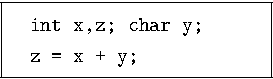
\includegraphics[width=0.45\textwidth]{typeErr-crop.pdf}}
  &
\multicolumn{1}{m{0.5\textwidth}}{
\greentext{\small\texttt{+}の両辺の型が違うとき，構文的に正しくても
有効な命令に変換可能か？}}
\end{tabular}
\end{frame}

\begin{frame}[fragile]
  \frametitle{型定義}

  $T$は，整数($\mathsf{integer}$)か浮動小数点数($\mathsf{float}$)の変数型，および，
  その配列の型を生成する．例：\verb|int[2][3]|, \verb|float[10]|

  \[\begin{array}{l|p{0.5\textwidth}}
    \mbox{生成規則} & \mbox{意味ルール}\\\hline
    T \rightarrow B\;C & $T.t=B.t$, $C.b=B.t$\\ 
    B \rightarrow \mathbf{int} & $B.t=\mathsf{integer}$\\
    B \rightarrow \mathbf{float} & $B.t=\mathsf{float}$\\
    C \rightarrow \texttt{[}\,\mathbf{num}\,\texttt{]}C_1 & $C.t=array(\mathsf{number}.val,C_1.t)$\\
    & $C_1.b=C_b$\\
    C \rightarrow \varepsilon & $C.t=C.b$
  \end{array}\]

  \begin{list}{}{}
  \item \verb|int[2][3]|が割り当てる領域 32bit$\times$6
  \item \verb|float[10]|が割り当てる領域 64bit$\times$10
  \end{list}
  配列の大きさは予め決定されている必要がある：駆動レコード，ヒープのため
\end{frame}

\begin{frame}
  \frametitle{型整合性}
  型が一致しない場合の対応はプログラミング言語ごとに異なる．

  \begin{itemize}
    \item 型が一致しない場合はエラーとする．\\
    型ごとに演算を用意する．MLの\texttt{+}(整数)と\texttt{+.}(固定小数点)\\
    OCaml, Haskell, C, Javaなど
    \item 型変換する．\\
    型キャストによって明示的に変換するか，暗黙的に変換する．
    部分型の定義によって柔軟に適用させるようにする．\\
    Lisp, SmallTalk, Perlなど
  \end{itemize}
  
型チェック：
\begin{itemize}
  \item {\bf 静的型チェック}\quad
  コンパイル時に型整合性を検査して，型が合わない場合はコード生成しない．
  \item {\bf 動的型チェック}\quad
  コンパイル時は整合性を厳しく検査せず，実行時にできるだけ型が合うように実行する．
\end{itemize}

\end{frame}

\begin{frame}[fragile]
  \frametitle{多相型とオーバーロード}

  \begin{itemize}
  \item 多相型(polymorphism)：リストなど共通の操作を持つデータ型
  
  Listはその要素の型にかかわらず同じ性質を持つ．\\
  結合(append)，先頭要素(head)，先頭を除いたリスト(tail)，i番目の取り出し(i-th) etc.

  \vspace*{10pt}

  型変数を持つデータ型:\verb|List<X>|

  型変数に具体的なデータ型を適用して，データ型を構成する．

  整数リスト＝\verb|List<Int>|, 文字リスト＝\verb|List<Char>|

  \item オーバーロード：異なる型に対して同じ操作を認める
  
  加算：整数，実数などに対して同じ記号\texttt{+}を用いる

  \texttt{x+y}は，$x$,$y$の型に応じて操作を切り替える．
  \begin{trivlist}
  \item $\texttt{x}$, $\texttt{y}$がともに整数の場合：整数の加算
  \item $\texttt{x}$, $\texttt{y}$がともに実数の場合：実数の加算
  \end{trivlist}
  \greentext{言語によってはオーバーロードなし：MLにおける \texttt{+}と\texttt{+.}}
\end{itemize}
\end{frame}

\end{document}
